\documentclass{beamer}

\usepackage[slovene]{babel}
\usepackage[utf8]{inputenc}
\usepackage{amsfonts,amssymb}
\usepackage{theorem}
\usepackage{array}
\usepackage{amsfonts}
\usepackage{pifont}

\usepackage{graphicx}
\graphicspath{ {slike/} }

\newcommand{\cmark}{\ding{51}}
\newcommand{\xmark}{\ding{55}}

\usetheme{Berkeley}

\title{Kodiranje s pomočjo sudoku ključa}
\author{Klementina Pirc}
\institute{Fakulteta za matematiko in fiziko \\ Oddelek za matematiko}
\date{26. april 2018}

\begin{document}

%%%%%%%%

\begin{frame}
\titlepage
\end{frame}

%%%%%%%%

% UVOD
\section{Uvod}

%%%%%%%%

\begin{frame}{Uvod}
\begin{itemize}
\item varovanje podatkov
\item prednost kvantnega šifriranja
\end{itemize}
\end{frame}

%%%%%%%%

% POLARIZACIJA FOTONOV
\section{Polarizacija fotonov}

%%%%%%%%

\begin{frame}{Polarizacija fotonov}

\begin{block}{Definicija}
Osnovni delec je delec ki nima podstrukture, torej ni sestavljen iz manjših delcev.
\end{block}

\begin{block}{Definicija}
Svetloba je elektromagnetno valovanje pri različnih valovnih dolžinah oziroma frekvencah.
\end{block}

\begin{block}{Definicija}
Foton je brezmasni in električno nevtralen osnovni delec, ki potuje s svetlobno hitrostjo in je osnovni gradnik svetlobe.
\end{block} 

\end{frame}

%%%%%%%%

\begin{frame}{Polarizacija valovanja}

\begin{block}{Definicija}
Polarizacija valovanja opisuje smer nihanja količine ki valuje.
\end{block}

\begin{figure}
\centering
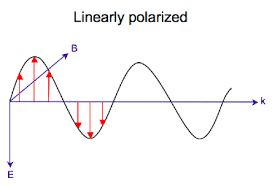
\includegraphics[scale=0.75]{images}
\end{figure}

\end{frame}

%%%%%%%%

\begin{frame}{Osnovne polarizacije}

\begin{block}{Definicija}
Val je linarno polariziran, če nihanje poteka le v eni smeri. Krožno in eliptično polarizacijo dobimo, kadar se s širjenjem vala nihanje suče.
\end{block}

\begin{figure}
\centering

\includegraphics[scale=2]{polcls}
\end{figure}

\end{frame}

%%%%%%%%

\begin{frame}{Elektromagnetno valovanje}

\begin{figure}
\centering
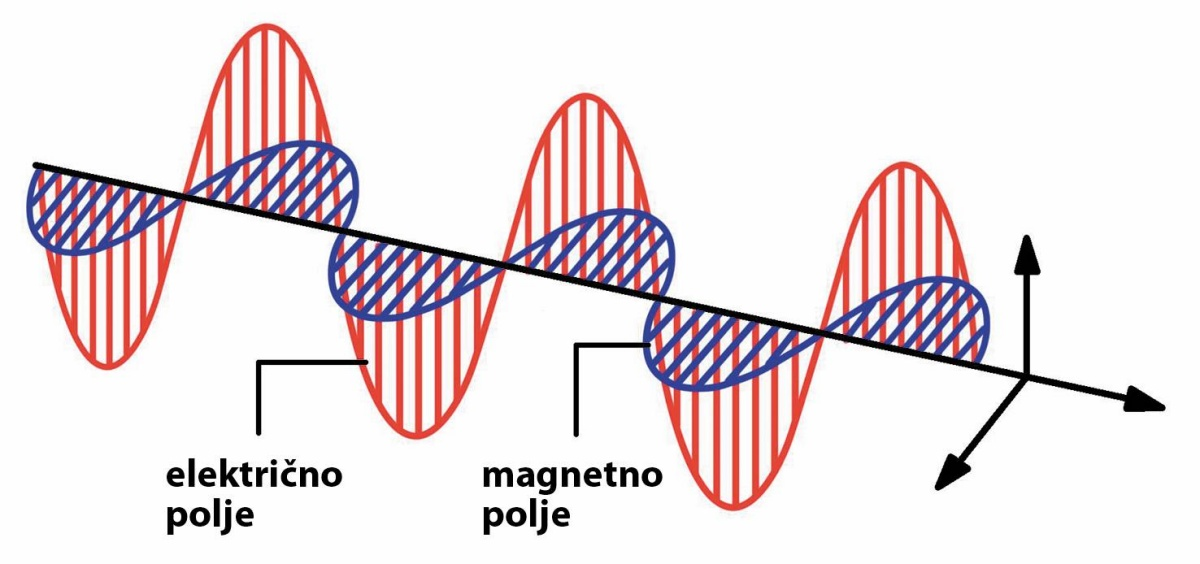
\includegraphics[scale=0.75]{emv}
\end{figure}

\begin{block}{Dogovor}
Smer polarizacije je enaka smeri nihanja jakosti električnega polja.
\end{block}

\end{frame}

%%%%%%%%

\begin{frame}{Polarizator}

\begin{block}{Definicija}
Polarizator je naprava, ki valovanje z nedoločeno ali mešano polarizacijo spremeni v valovanje z določeno polarizacijo.
\end{block}

\begin{figure}
\centering
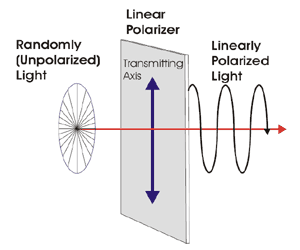
\includegraphics[scale=0.6]{linear-figure-1}
\end{figure}

\end{frame}

% KVANTNA RAZDELITEV KLJUČA
\section{Kvantna razdelitev ključa}

%%%%%%%%

\begin{frame}{Kvantna razdelitev ključa}

\begin{block}{Definicija}
Šifriranje podatkov je pretvorba podatkov v obliko, ki je nepooblaščene osebe ne razumejo.
\end{block}

\begin{block}{Definicija}
Alica je pošiljatelj sporočila,\\
Bob sporočilo prejme,\\
Eva pa ga skuša prestreči, torej je prisluškovalka.
\end{block}

\end{frame}

%%%%%%%%

\begin{frame}{Zaporedje polariziranih fotonov}

Vrednost in ustrezna polarizacija:\\ \medskip
\begin{tabular}{l c c}
vrednost & 0 & 1\\
polarizacija & $\rightarrow$ & $\uparrow$\\
\end{tabular} \\

\bigskip

Število v binarnem zapisu kot zaporedje polariziranih fotonov:\\ \medskip
\begin{tabular}{l c c c c c}
vrednost & 1 & 0 & 1 & 1 & 0\\
polarizacija & $\uparrow$ &  $\rightarrow$ & $\uparrow$ & $\uparrow$ &  $\rightarrow$\\
\end{tabular}

\end{frame}

%%%%%%%%

\begin{frame}{Prejemanje polariziranih fotonov}

\begin{tabular}{l c c c c}
vrednost & 1 & 0 & 1 & 0\\
polarizacija & $\uparrow$ & $\rightarrow$ & $\nwarrow$ & $\nearrow$\\
baza polarizacije & + & + & $\times$ & $\times$\\
\end{tabular}

\bigskip

\begin{tabular}{ l m{0.2 cm} m{0.2 cm} m{0.2 cm} m{0.2 cm} m{0.2 cm} m{0.2 cm} m{0.2 cm} m{0.2 cm} m{0.2 cm} m{0.2 cm} m{0.2 cm} m{0.2 cm}}
Alica\\
vrednost & 1 & 0 & 1 & 1 & 0 & 0 & 1 & 1 & 0 & 0 & 1 & 1 \\
polarizacija & $\uparrow$ & $\rightarrow$ & $\nwarrow$ & $\uparrow$ & $\nearrow$ & $\nearrow$ & $\nwarrow$  & $\uparrow$ & $\nearrow$ & $\rightarrow$ & $\uparrow$ & $\nwarrow$\\
baza & + & + & $\times$ & + & $\times$ & $\times$ & $\times$ & + & $\times$ & + & + & $\times$\\
\\
Bob\\
baza & + & $\times$ & + & + & $\times$ & $\times$ & + & + & $\times$ & + & $\times$ & $\times$\\
polarizacija & $\uparrow$ & $\nearrow$ & $\rightarrow$ & $\uparrow$ & $\nearrow$  & $\nearrow$ & $\uparrow$ & $\uparrow$ & $\nearrow$ & $\rightarrow$ & $\nearrow$ & $\nwarrow$\\
vrednost & 1 & 0 & 0 & 1 & 0 & 0 & 1 & 1 & 0 & 0 & 0 & 1\\
\\
ključ & 1 & - & - & 1 & 0 & 0 & - & 1 & 0 & 0 & - & 1\\
\end{tabular}

\end{frame}

%%%%%%%%

\begin{frame}{Primer prisluškovalca}

\begin{tabular}{ l m{0.3 cm} m{0.3 cm} m{0.3 cm} m{0.3 cm} m{0.3 cm} m{0.3 cm} m{0.3 cm} m{0.3 cm}}
vrednost & 0 & 1 & 1 & 0 & 1 & 0 & 0 & 1\\
polarizacija & $\rightarrow$ & $\uparrow$ & $\nwarrow$ & $\rightarrow$ & $\nwarrow$ & $\nearrow$ & $\nearrow$  & $\uparrow$\\
baza polarizacije & + & + & $\times$ & + & $\times$ & $\times$ & $\times$ & + \\
\\
Evin polarizator & + & $\times$ & + & + & $\times$ & + & $\times$ & +\\
nova polarizacija & $\rightarrow$ & $\nearrow$ & $\uparrow$ & $\rightarrow$ & $\nwarrow$  & $\uparrow$ & $\nearrow$ & $\uparrow$\\
\\
Bobov polarizator & + & $\times$ & $\times$ & $\times$ & + & $\times$ & + & +\\
odčitana polarizacija & $\rightarrow$ & $\nearrow$ & $\nearrow$ & $\nwarrow$ & $\uparrow$  & $\nearrow$ & $\rightarrow$ & $\uparrow$\\
odčitana vrednost & 0 & 0 & 0 & 1 & 1 & 0 & 0 & 1\\
\\
končni ključ & 0 & - & 0 & - & - & 0 & - & 1\\
ujemanje ključev & \cmark & - & \xmark & - & - & \cmark & - & \cmark\\ 
\end{tabular}

\end{frame}

%%%%%%%%

% SUDOKU
\section{Sudoku}

%%%%%%%%

\begin{frame}{Sudoku}

\begin{block}{Definicija}
Sudoku je logična uganka, pri kateri je cilj zapolniti mrežo velikosti 9x9 s števili od 1 do 9 tako, da se vsako število v vsakem stolpcu, vrstici in 3x3 kvadratu znotraj mreže pojavi natanko enkrat.
\end{block}

\begin{figure}
\centering
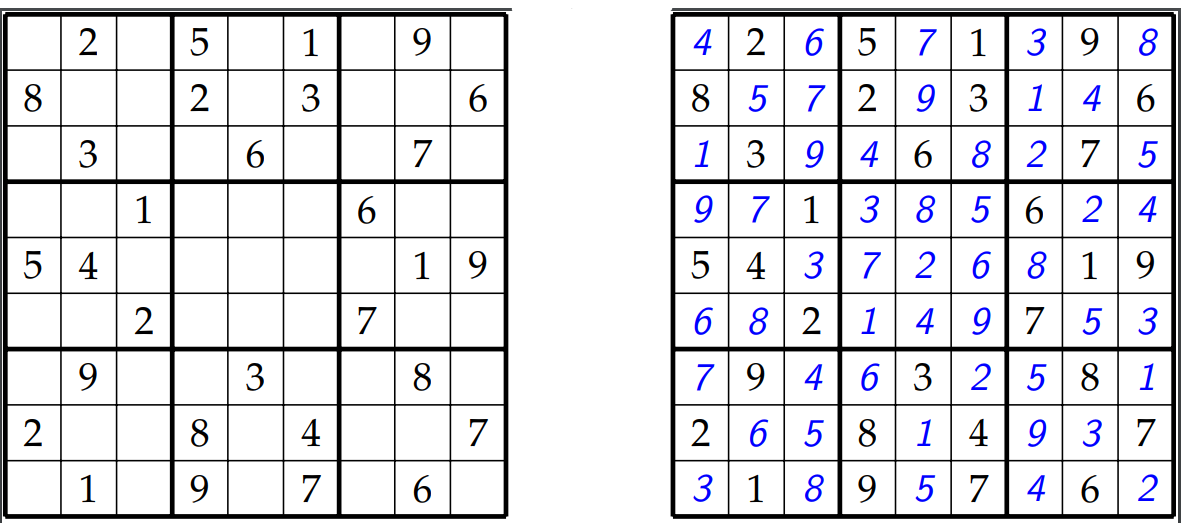
\includegraphics[scale=0.3]{sudoku_resen}
\end{figure}

\end{frame}

%%%%%%%%

\begin{frame}{Lastnosti sudokuja}

\begin{itemize}
\item Howard Garns (1979)
\item 6.670.903.752.021.072.936.960 mrež velikosti 9x9
\item težavnost
\item problem najmanjšega števila podanih števil
\item Sudoku X, geometrijski sudoku
\end{itemize}

\begin{figure}
\centering
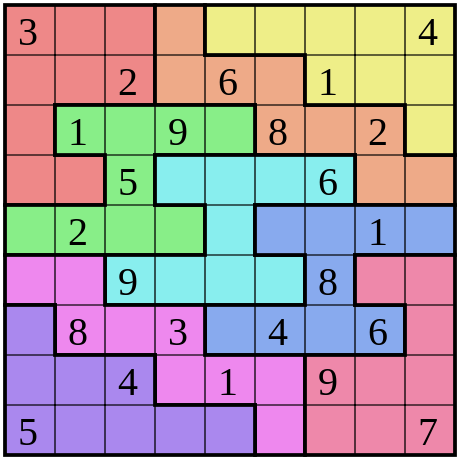
\includegraphics[scale=0.23]{geo_sudoku}
\end{figure}

\end{frame}

%%%%%%%%

% SUDOKU KLJUČ
\section{Sudoku ključ}

%%%%%%%%

\begin{frame}{Sudoku ključ}

\begin{columns}

\begin{column}{0.3\textwidth}

Izbran sudoku:\\

\begin{center}
\begin{tabular}{| c | c || c | c |}
\hline
0 & 1 & 2 & 3\\
\hline
3 & 2 & 1 & 0\\
\hline
\hline
2 & 0 & 3 & 1\\
\hline
1 & 3 & 0 & 2\\
\hline
\end{tabular}
\end{center}

\end{column}


\begin{column}{0.7\textwidth}

Izbrane polarizacije: \bigskip

\begin{tabular}{l c c c c}
vrednost & 0 & 1 & 2 & 3\\
polarizacija & $\rightarrow$ & $\uparrow$ & $\nwarrow$ & $\nearrow$\\
baza polarizacije & + & + & $\times$ & $\times$\\
\end{tabular}

\end{column}

\end{columns}

\bigskip

\begin{tabular}{m{1.5cm} m{0.10 cm} m{0.10 cm} m{0.10 cm} m{0.10 cm} m{0.10 cm} m{0.10 cm} m{0.10 cm} m{0.10 cm} m{0.10 cm} m{0.10 cm} m{0.10 cm} m{0.10 cm} m{0.10 cm} m{0.10 cm} m{0.10 cm} m{0.10 cm}}
Alica\\
vrednost & 0 & 1 & 2 & 3 & 3 & 2 & 1 & 0 & 2 & 0 & 3 & 1 & 1 & 3 & 0 & 2\\
polarizacija & $\rightarrow$ & $\uparrow$ & $\nwarrow$ & $\nearrow$ & $\nearrow$ & $\nwarrow$ & $\uparrow$ & $\rightarrow$ & $\nwarrow$ & $\rightarrow$ & $\nearrow$ & $\uparrow$ & $\uparrow$ & $\nearrow$ & $\rightarrow$ & $\nwarrow$\\
baza & + & + & $\times$ & $\times$ & $\times$ & $\times$ & + & + & $\times$ & + & $\times$ & + & + & $\times$ & + & $\times$\\
\\
Bob\\
baza & + & $\times$ & + & + & $\times$ & $\times$ & + & $\times$ & + & $\times$ & $\times$ & + & $\times$ & $\times$ & $\times$ & $\times$\\
vrednost & 0 & . & . & . & 3 & 2 & 1 & . & . & . & 3 & 1 & . & 3 & . & 2\\ 
\end{tabular}

\end{frame}

%%%%%%%%


\end{document}